\documentclass[11pt]{article}
\usepackage[margin=1in]{geometry}
\usepackage{amsmath,amsfonts,amssymb}
\usepackage{graphicx}
\usepackage{float}
\usepackage{array}
\usepackage{listings}
\usepackage{url}
\usepackage{xcolor}

\definecolor{codegreen}{rgb}{0,0.6,0}
\definecolor{codegray}{rgb}{0.5,0.5,0.5}
\definecolor{codepurple}{rgb}{0.58,0,0.82}
\definecolor{backcolour}{rgb}{0.95,0.95,0.92}

\lstdefinestyle{mystyle}{
    backgroundcolor=\color{backcolour},   
    commentstyle=\color{codegreen},
    keywordstyle=\color{magenta},
    numberstyle=\tiny\color{codegray},
    stringstyle=\color{codepurple},
    basicstyle=\ttfamily\footnotesize,
    breakatwhitespace=false,         
    breaklines=true,                 
    captionpos=b,                    
    keepspaces=true,                 
    numbers=left,                    
    numbersep=5pt,                  
    showspaces=false,                
    showstringspaces=false,
    showtabs=false,                  
    tabsize=2
}

\lstset{style=mystyle}

\graphicspath{{images/}}

\title{Project 3 - Control Systems Design - Fall 2021}
\author{Alan Chacko}
\date{12/21/2021}

\begin{document}
\maketitle

\section*{Project Formulation}

Utilizing the nonlinear mathematical model of the system that represents dynamics of human bone marrow production of neutrophils under the suppressive impact of chemotherapy, derived by Friberg et al. [1]-[2], we can define an optimal chemotherapy drug dosing schedule for maintaining a pre-specified neutrophil level in patients.

The variable optimal amounts of daily drug administration ($Edrug$) is adjusted according to feedback information on the actual count of neutrophils ($ACN$). We utilize the nonlinear Friberg's model provided in [1] to generate a linear model to analyze. 

In the first part of this paper, we analyze the general characteristics of the model itself without feedback, and observe the changes in neutrophil levels when constant drug dosages are administered daily.

In the second part of the paper, we design an LQR feedback controller to variably adjust $Edrug$ to ensure the neutrophil level approaches but does not dip below a predefined $ACN$ level of $1.5\times 10^9$ neutrophils.

\section*{Part 1: System Analysis of Friberg's Model}

To model the change in neutrophils over time after constant drug administration, we can use the following block diagram to simulate the nonlinear system.

\begin{figure}[H]
    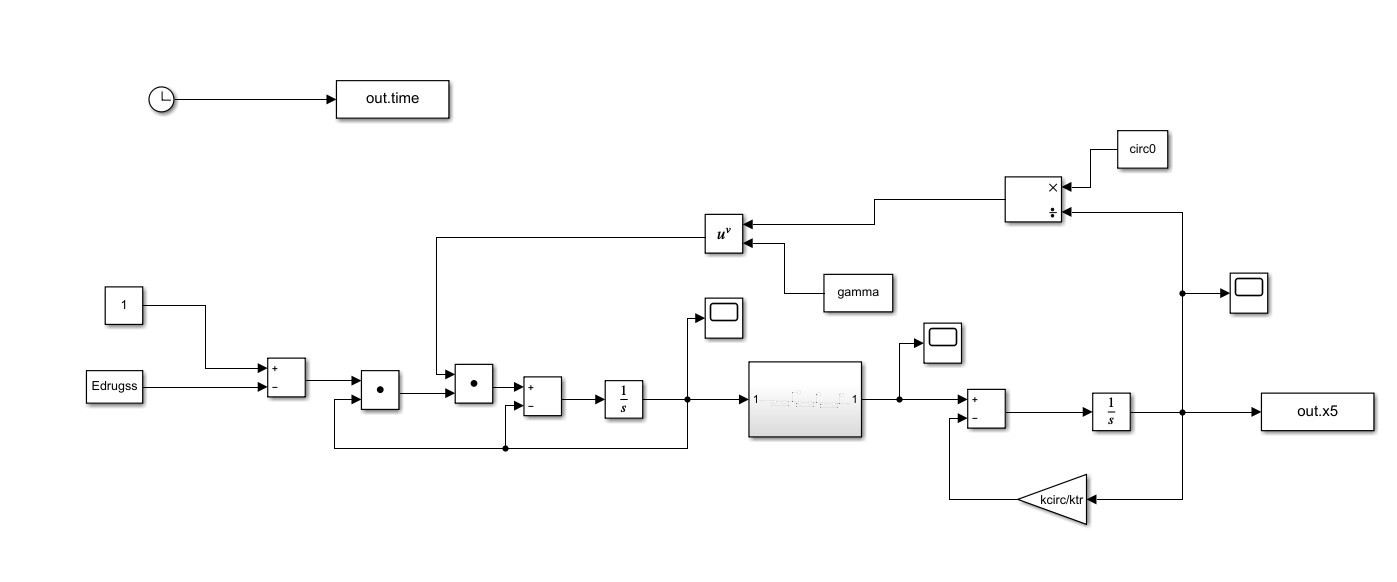
\includegraphics[width=\textwidth]{p1blockdiagram.jpg}
\end{figure}

All constants used in the model are predefined:

$$
Circ_0 = 5.04\times 10^9 \frac{1}{L}, \quad k_{tr} = k_{prol} = k_{circ} = 0.0332 \frac{1}{h}, \quad \gamma = 0.16, \quad ANC = 1.5\times 10^9 \frac{1}{L}
$$

Note the neutrophil values used in the model are scaled down by a factor of $10^9$. 

Under a constant administrated drug concentration, we can analyze the change in the number of neutrophils over a period of 50 days. Below is an example plot of the change in neutrophil levels over 50 days when 250mg are administered daily.

\begin{figure}[H]
    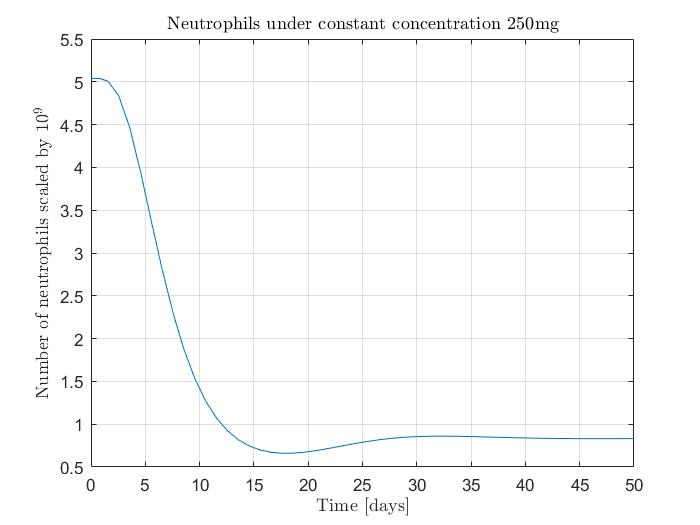
\includegraphics[width=\textwidth]{p1image1.jpg}
\end{figure}

If instead we are given a pre-specified neutrophil count to reach, as defined by the variable $ANC$, we can link this value to the required steady-state dosage for the system, using a parameter $\alpha$ that is betweeen 1 and $\alpha_{max} = Circ_0/ANC = 3.35$. So the equation is:

$$
E_{Drug}^{ss} = 1 - (\frac{\alpha \times ANC}{\alpha_{max} \times ANC})^{\gamma}
$$

In the plot below, given an $ANC = 1.5$ and an $\alpha = 1$, we require:

$$
E_{Drug}^{ss} = 1 - (0.2998)^{0.16} = 0.1763
$$

\begin{figure}[H]
    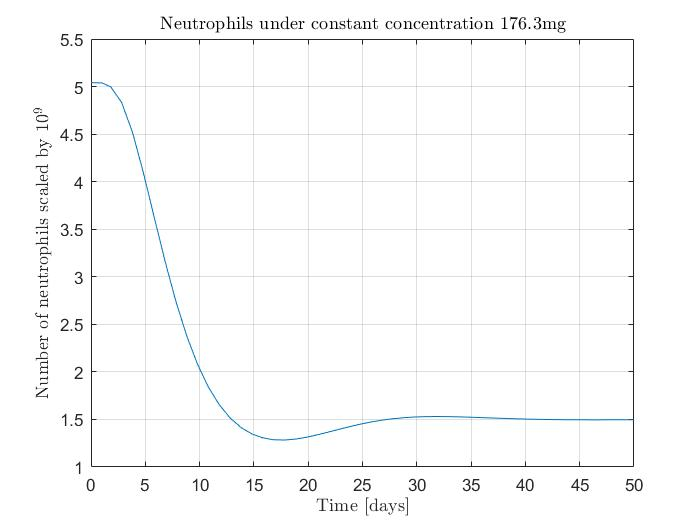
\includegraphics[width=\textwidth]{p1image2.jpg}
\end{figure}

\section*{Part 2: Optimal Dosing}

A constraint during chemotherapy administration is that the absolute neutrophil count ($ANC$) should stay above the limit that defines neutropenia.

After linearizing Friberg's model, we apply LQR to find an optimal gain $F$ using the given linearized model state-space matrices $A$ and $B$, and given optimal quadratic regulator values $R_1$ and $R_2$. 

We can adjust $R_1$ to penalize certain states over others. We can penalize actions that can lead to an overshoot below the specified ($ANC$). $R_1$ is a 5x5 diagonal matrix.

To control the rate of stabilization, we specify $R_2$ to be relatively large at $R_2 = 25$. This value allows the model to reach $ANC$ before the 15th day.

By using the MATLAB lqr function, we can generate a gain vector $F_{opt}$.

The $F_{opt}$ assumes that $x_{1ss} = ANC$ and all other steady states are $Circ_0 = x_{5ss} = x_{4ss} = x_{3ss} = x_{2ss}$, 

$$
F_{opt} = \begin{bmatrix}
    -2.0148 & -0.0446 & -0.0306 & -0.0030 & 0.0710
\end{bmatrix}
$$

With the given $F_{opt}$, we can now build the block diagram to simulate the system. $F_{opt}$ provides feedback on the direction drug concentration needs to be adjusted for us to smoothly reach the desired $ANC$ based on the error between the current state ($\dot{x}(t)$) and defined steady state values ($\dot{x}_{ss}$).

The image of the block diagram is below:

\begin{figure}[H]
    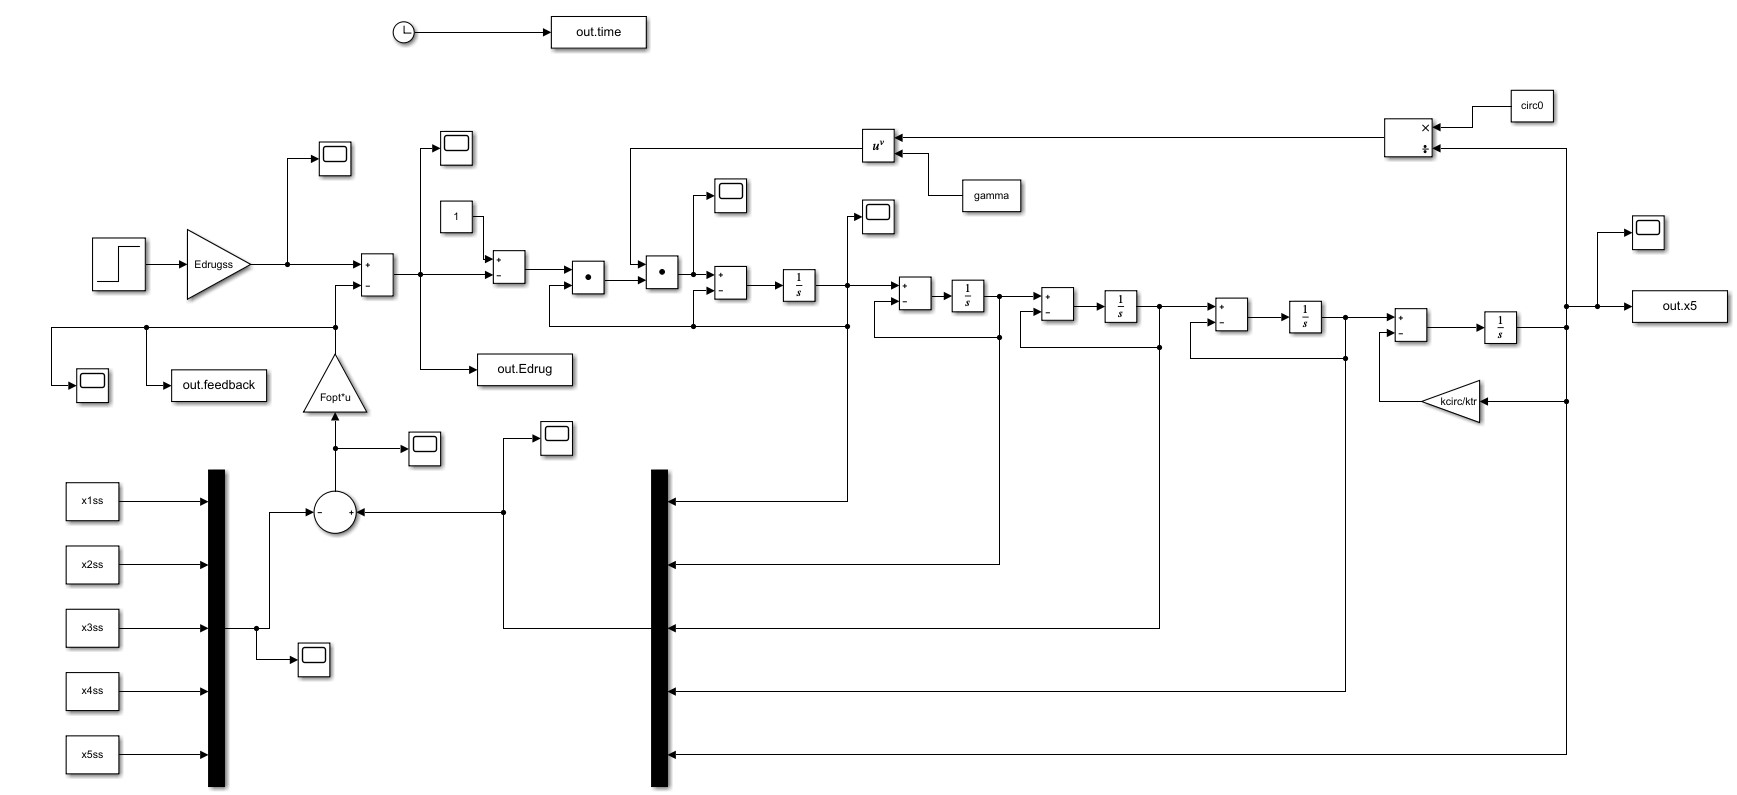
\includegraphics[width=\textwidth]{p2blockdiagram.jpg}
\end{figure}


We can then plot the number of neutrophils over a 15-day interval:

\begin{figure}[H]
    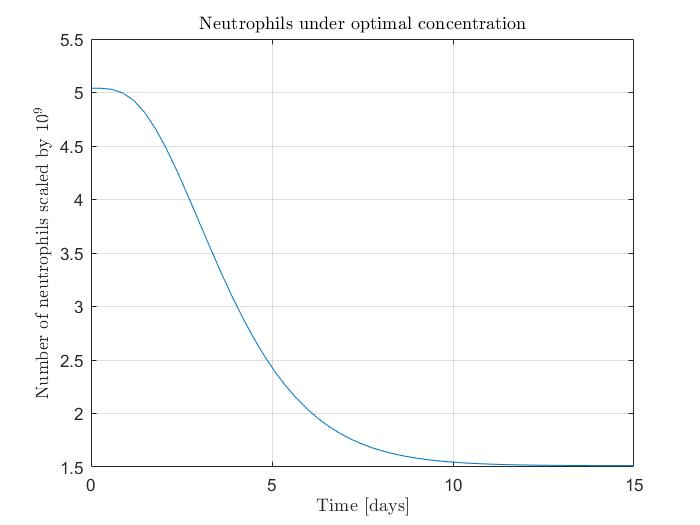
\includegraphics[width=\textwidth]{p2image1.jpg}
\end{figure}

And then plot the optimal continuous drug schedule based on the above 15-day interval:

\begin{figure}[H]
    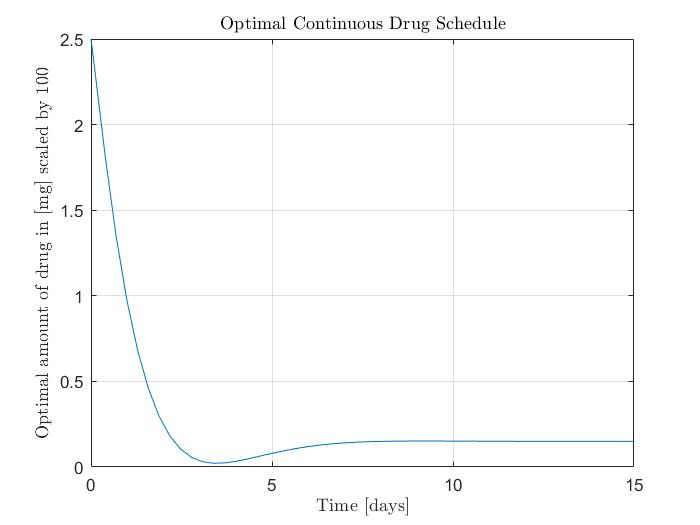
\includegraphics[width=\textwidth]{p2image2.jpg}
\end{figure}

\section*{Conclusions}

In summary, we can design a model for an optimal dosing schedule that allows us to target a specific neutrophil level using LQR. LQR can keep neutrophil levels stable during decline and prevent us from overshooting the target level.

\begin{thebibliography}{3}
  \bibitem{ref1} L. E. Friberg, A. Henningsson, H. Mass, L. Nguyen, and M. O. Karlsson: Model of chemotherapy-induced myelosuppression with parametric consistency across drugs. Journal of Clinical Oncology 20: 4713-4721, 2002.
  \bibitem{ref2} L. E. Friberg and M. Karlsson: Mechanistics models for myelosuppression. Investigational New Drugs 21:183-194, 2003
  \bibitem{ref3} Y. Guo, N. Haddish-Berhane, H. Xie, and D. Ouellet: Optimization of clinical dosing schedule to manage neutropenia: learning from semi-mechanistic modeling simulation approach. Journal of Pharmacokinetics and Pharmacodynamics 47: 47-58, 2020.
  \bibitem{ref4} V. Radisavljevic-Gajic: Linear-quadratic (LQ) optimal steady state controllers for engineering
  students and practicing engineers. International Journal of Mechanical Engineering Education:
  49, 316-358, 2021.
\end{thebibliography}

\section*{Appendix: Project Code}

\lstinputlisting[language=Matlab]{../project3.m}

\end{document}